\documentclass[conference]{IEEEtran}
% If the IEEEtran.cls has not been installed into the LaTeX system files, 
% manually specify the path to it:
% \documentclass[conference]{../sty/IEEEtran} 
\usepackage[brazil]{babel}
\usepackage{amsmath}
\usepackage{multirow}
\usepackage[utf8]{inputenc}
\usepackage[T1]{fontenc}
\usepackage{graphicx}

% correct bad hyphenation here
\hyphenation{op-tical net-works semi-conduc-tor IEEEtran}

\begin{document}
	
	% paper title
	\title{Redes Neurais Artificiais: Artigo 2}
	
	
	% author names and affiliations
	% use a multiple column layout for up to three different
	% affiliations
	\author{\authorblockN{Victor São Paulo Ruela \\}
		\authorblockA{Programa de Pós-Graduação em Engenharia Elétrica\\
			Universidade Federal de Minas Gerais\\
			Belo Horizonte, Brasil\\
            Email: victorspruela@ufmg.br}}
	
	% avoiding spaces at the end of the author lines is not a problem with
	% conference papers because we don't use \thanks or \IEEEmembership
	
	% use only for invited papers
	%\specialpapernotice{(Invited Paper)}
	
	% make the title area
	\maketitle
	
	\begin{abstract}
		Este trabalho tem como objetivo avaliar o desempneho de diferentes modelos de redes neurais artificiais estudados durante a disciplina sobre bases de dados de benchmark presentes na literatura. Serão considerados o Perceptron, Adaline, Redes RBF, ELM e ELM com aprendizado Hebbiano. Para três problemas de regressão e classificação binária escolhidos, um experimento foi desenhado seguindo as recomendações da literatura. Os resultados de cada modelos são comparados por meio de testes estatíscticos para as metrícas AUC (classficação) e coeficiente de correlação linear (regressão). Os resultados mostraram que ...
	\end{abstract}

	\section{Introdução}
	A Rede Neural Artificial (RNA) é uma classe de modelos muito popular em problemas de classificação, reconhecimento de padrões, regressão e predição~\cite{jain1996artificial}. Inspirado pelas características do cérebro humano, elas possuem como elementos básicos neurônios artificiais capazes de executar operações matemáticas, representando desta forma modelos de neurônios biológicos. Através de sua organização em diferentes estruturas de rede, tais modelos são capazes de se adaptar e representar funções matemáticas bastante complexas. 

	\section{Revisão da literatura}
	Nesta seção é feita uma breve descrição dos modelos de redes neurais utilizados neste trabalho.
	
	\subsection{Perceptron}
	Proposto inicialmente por Rosenblatt~\cite{rosenblatt1957perceptron}, este é um modelo geralmente utilizado para a solução de problemas de classificação lineares. No seu trabalho original, o autor descreve formas de adaptação dos parâmetros, ou pesos, da rede com o objetivo de reduzir a discrepância entre as saídas esperadas e estimadas e aprender associações entre os neurônios, o que é a base da indução para diversos algoritmos atuais. Este trabalho é considerado um marco na literatura por diversos autores.
	
	Se considerarmos uma função de ativação contínua e diferenciável, os pesos da rede poderão ser inferidos de forma explícita, através do cálculo da pseudo-inversa, ou pelo algoritmo do gradiente descendente~\cite{hertz1991introduction}. Exemplos de funções de ativação com esta característica frequentemente empregadas na literatura são a função logística, tangente hiperbólica e linear~\cite{jain1996artificial}. Vale a pena ressaltar que a covergência destas abordagens está condicionada aos dados utilizados para treinamento serem linearmente independentes~\cite{hertz1991introduction}.
	
	\subsection{Adaline}
	O Adaline foi inicialmente desenvolvido por Widrow em 1960~\cite{widrow1960adaptive}, sendo principamente aplicado em problemas de regressão lineares. Assim como o Perceptron, originalmente este modelo considera somente um neurônio MCP em sua formulação, entretando sua função de ativação é a identidade. Seu treinamento é formulado como um problema de otimização com custo quadrático, onde originalmente foi utilizado o algoritmo do gradiente descendente para sua solução. 
	
	Para este agoritmo, em cada iteração é dado um passo na direção oposta ao gradiente da função objetivo, resultanto em uma convergência gradual para o mínimo do problema. Este gradiente pode ser calculado de forma análitica para a estrutura de rede do Adaline, o qual é no fim proporcional à diferença entre os valores estimados e reais~\cite{widrow1960adaptive}, bastante similar ao Perceptron simples. É fácil notar que o treinamento também pode ser realizado de forma direta através do cálculo da pseudo-inversa dos dados de entrada, já que este é um problema de mínimos quadrados~\cite{haykin2007neural}.
	
	\subsection{Redes RBF}
	As redes RBF foram inicialmente introduzidas por~\cite{broomhead1988multivariablefi} e são caracterizadas por um aprendizado que envolve duas etapas: (i) aplicar uma transformação aos padrões para um espaço onde a probabilidade de serem linearmente separáveis é alta (ii) encontrar os pesos usando o estimador mínimos quadrados usado no Perceptron simples. Essa estrutura pode ser representada por um rede de três camadas, onde sua camada escondida é reponsável pela transformação não-linear das estradas para o novo espaço, geralmente para uma dimensão muito alta. 
	
	\subsection{ELM}	
	Inicialmente proposto por~\cite{huang2004extreme}, as máquinas de aprendizado extremo (ELM) são redes neurais com uma única camada escondida, as quais possuem o atrativo de poucos parâmetros a serem ajustados, generalização maior ou similar e redução do tempo de treinamento das redes em relação aos métodos convencionais. Seu treinamento é baseado na teoria de minimização de risco empírico, necessitando de somente uma iteração para este processo, evitando múltiplas iterações e algoritmos de otimização local~\cite{ding2015extreme}. 
	
	ELMs são capazes de definir adaptivamente o número neurônios da rede e aleatoriamente escolher os pesos das entradas e viéses da camada escondida~\cite{huang2006extreme}. Isso faz com o que a rede possa ser considerada como um sistema linear, o qual pode ser calculado de forma analítica através de uma operação de inversão da matriz de pesos da camada de saídas~\cite{huang2006extreme}. Essa característica permite uma drástica redução do esforço computacional do treinamento, geralmente de 10 vezes ou mais~\cite{deng2010research}. 
	
	\section{Metodologia}
	\subsection{Bases de Dados}
	Neste trabalho serão consideradas três bases de dados referentes a problemas de classificação binários e regressão multivariada disponíveis no repositório da UCI \cite{dua2019}, totalizando seis problemas. Antes do treinamento, os dados de entrada serão normalizados para o intervalo $[-1,1]$ e filtrados para remoção de valores inválidos.
	
	\subsection{Desenho do experimento}
	A partir das recomendações para desenho de experimento para comparação de algoritmos proposta em \cite{salzberg1997comparing}, a seguinte metodologia será adotada:
	\begin{itemize}
		\item Para cada base de dados:
			\begin{enumerate}
			\item Particionar os dados $D$ em $k$ partições para validação cruzada, mantendo a mesma proporção entre os rótulos
			\begin{enumerate}
				\item Criar o conjunto de treino $T = D - k$
				\item Para cada modelo:
				\begin{enumerate}
					\item Executar busca exaustiva com validação cruzada sobre $T$ para os coeficientes de regularização $\lambda$ \label{item:grid-search}
					\item Escolher $\lambda$ que obtém o melhor ajuste médio 
					\item Avaliar a métrica do modelo sobre $k$
				\end{enumerate}
			\end{enumerate}
			\item Estimar o intervalo de confiança do valor médio da métrica sobre $k$ usando \textit{bootstraping}
		\end{enumerate}
	\end{itemize}
	
	O número de partições consideradas será de $k=10$. Para o item \ref{item:grid-search}, serão considerados um número fixo de valores igualmente espaçados  dentro de um intervalo pré-definido. Além disso, serão considerados cinco partições para a validação cruzada, como forma de controlar um pouco o tamanho do experimento. Serão consideradas as métricas AUC e coeficiente de correlação linear $R^2$ para classificação e regressão, respectivamente.
	
	A implementação deste experimento, bem como dos modelos utilizados, será feita em Python e utilizando principalmente os pacotes \textit{numpy} \cite{harris2020array} e \textit{scikit-learn} \cite{scikit-learn}. O experimento será realizado em um Notebook Intel Core i7 Quad Core com 8Gb de memória RAM, sendo que o uso de paralelização será utilizado sempre que possível visto a enorme quantidade de vezes que os modelos serão treinados.
	
	\section{Resultados}
	
	\subsection{Problemas de Classificação}
	Para os problemas de classificação foram considerados os algoritmos Perceptron, RBF, ELM e ELM com apredizado Hebbiano. Foi estabelecido um número fixo de 20 neurônions na camada escondida e a regularização foi considerada somente para os algoritmos RBF e ELM. 50 valores de coeficiente de regularização foram escolhidos no intervalo $[0,1]$. O Perceptron foi executado com 100 épocas de treinamento e uma taxa de aprendizado de 0.01, não sido feito nenhum ajuste de hiper-parâmetros. Os gráficos boxplot para cada conjunto de dados considerado é exibido nas Figuras \ref{fig:box-statlog-heart}, \ref{fig:box-Climate-Model-Simluation} e \ref{fig:box-Liver-Disorder}.
	
	\begin{figure}[thpbh]
		\centering
		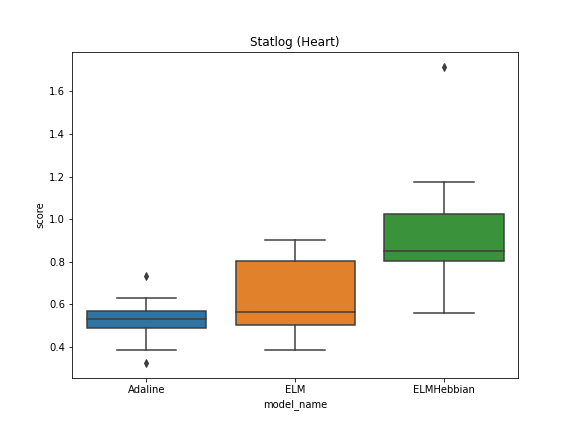
\includegraphics[width=0.5\textwidth]{figures/Statlog (Heart)_scores.png}
		\caption{Boxplots para a base de dados \textit{Statlog (Heart)}}
		\label{fig:box-statlog-heart}
	\end{figure}

	\begin{figure}[thpbh]
		\centering
		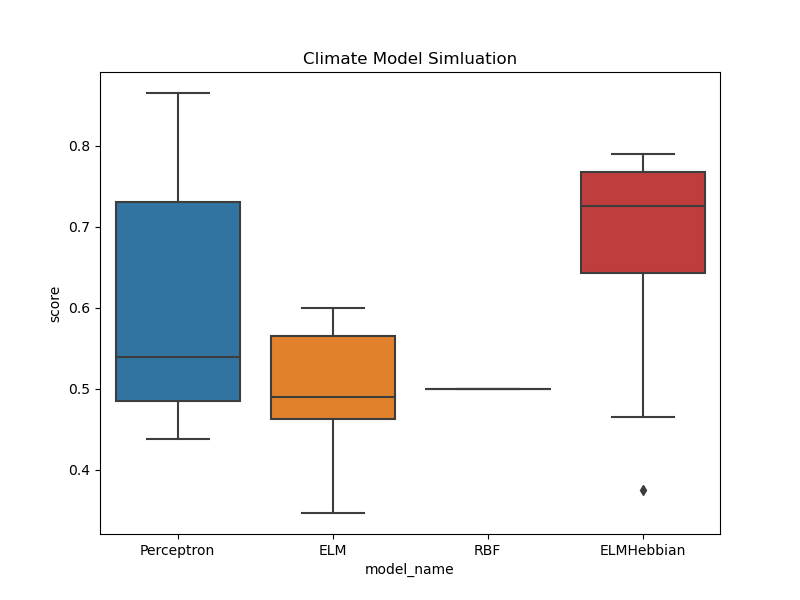
\includegraphics[width=0.5\textwidth]{figures/Climate Model Simluation_scores.png}
		\caption{Boxplots para a base de dados \textit{Climate Model Simulation}}
		\label{fig:box-Climate-Model-Simluation}
	\end{figure}

	\begin{figure}[thpbh]
		\centering
		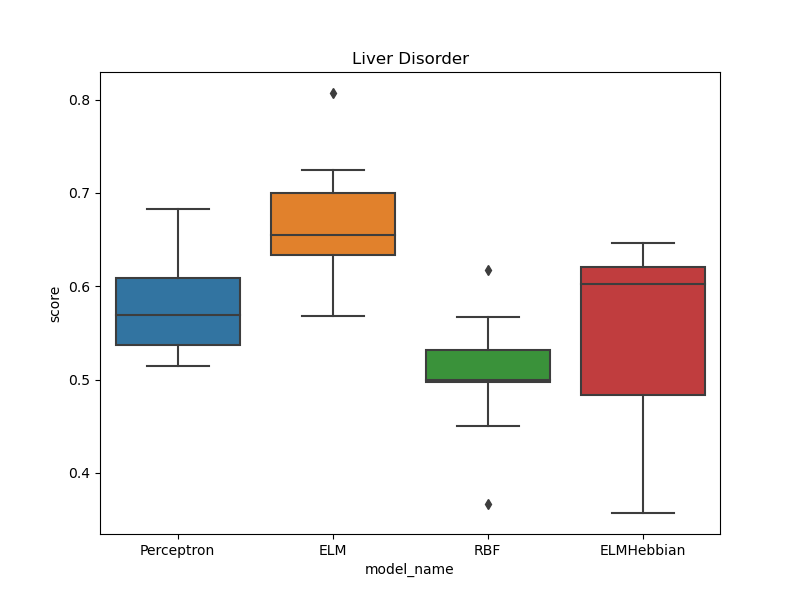
\includegraphics[width=0.5\textwidth]{figures/Liver Disorder_scores.png}
		\caption{Boxplots para a base de dados \textit{Liver Disorder (Bupa)}}
		\label{fig:box-Liver-Disorder}
	\end{figure}	
		
	
	\subsection{Problemas de Regressão}
	Para os problemas de classificação foram considerados os algoritmos Adaline, RBF e ELM. Não foi possível realizar uma implementação do ELM Hebbiano que funcionasse com problemas de regressão, logo este modelo teve que ser descartado. Foi estabelecido um número fixo de 20 neurônions na camada escondida e a regularização foi considerada somente para os algoritmos RBF e ELM. 50 valores de coeficiente de regularização foram escolhidos no intervalo $[0,1]$. O Adaline foi executado com 100 épocas de treinamento e uma taxa de aprendizado de 0.01, não sido feito nenhum ajuste de hiper-parâmetros. Os gráficos boxplot para cada conjunto de dados considerado é exibido nas Figuras \ref{fig:box-Boston-Housing}, \ref{fig:box-Parkinsons} e \ref{fig:box-Airfoil-Noise}.

	\begin{figure}[thpbh]
		\centering
		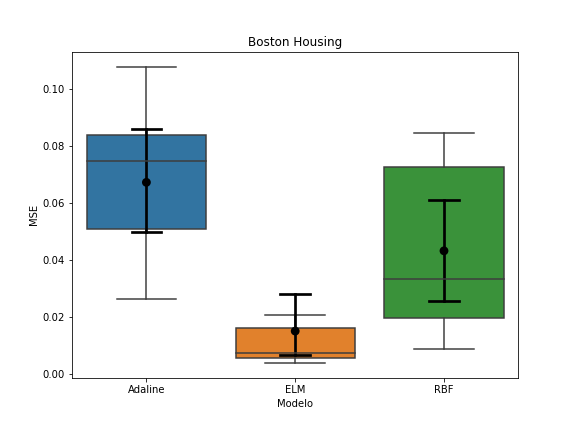
\includegraphics[width=0.5\textwidth]{figures/Boston Housing_scores.png}
		\caption{Boxplots para a base de dados \textit{Boston Housing}}
		\label{fig:box-Boston-Housing}
	\end{figure}
	
	\begin{figure}[thpbh]
		\centering
		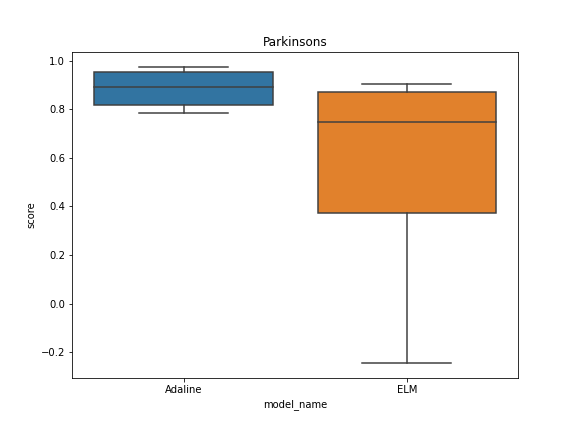
\includegraphics[width=0.5\textwidth]{figures/Parkinsons_scores.png}
		\caption{Boxplots para a base de dados \textit{Parkinsons}}
		\label{fig:box-Parkinsons}
	\end{figure}
	
	\begin{figure}[thpbh]
		\centering
		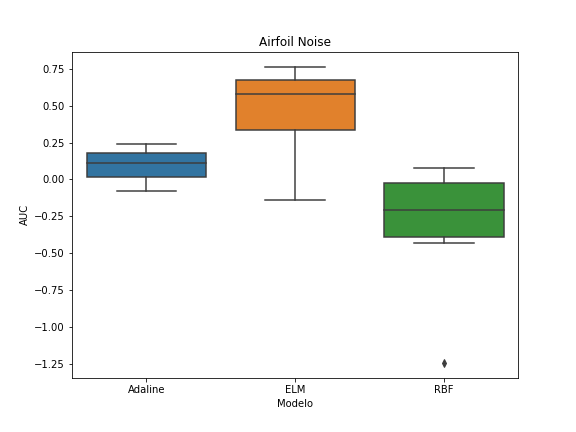
\includegraphics[width=0.5\textwidth]{figures/Airfoil Noise_scores.png}
		\caption{Boxplots para a base de dados \textit{Airfoil Noise}}
		\label{fig:box-Airfoil-Noise}
	\end{figure}	
	
	\section{Conclusões}
	
	Neste trabalho foi feita uma revisão bibligráfica de alguns dos principais trabalhos sobre redes neurais aritificiais. Realizando a divisão entre modelos para aprendizado supervisionado e não-supersvisionado, os conceitos básicos dos modelos estudados foram apresentados para contextualização, bem como uma breve análise das principais evoluções e aplicações propostas na literatura. Cada um destes modelos possui uma enorme quantidade de trabalhos publicados, portanto é de se esperar que publicações importantes tenham sido omitidos.
	
	Um aspecto não muito abordado neste trabalho foram as aplicações de RNAs, dado que o foco deste trabalho foi em entender um pouco mais de sua teoria. Em~\cite{abiodun2018state} está disponível uma lista das diferentes áreas em que RNAs são comumente aplicadas. Conforme observado durante a realização deste trabalho, grande partes das evoluções visam aprimorar eficiência dos algoritmos treinamento. Isso também é observado por~\cite{abiodun2018state}, o qual considera uma tendência trabalhos futuros visando aprimorar este aspecto.


    \bibliographystyle{unsrt}
	\bibliography{artigo2}
	
\end{document} 